%!TEX TS-program = XeLaTeX

%!TEX TS-program = XeLaTeX
\documentclass[11pt]{article}

\usepackage{amssymb}
\usepackage{amsthm}
\usepackage{amsmath}
\usepackage{mathtools}

\usepackage{fancyhdr}
\usepackage{graphicx}
\usepackage[top=3cm, left=2cm, right=2cm, headheight = 90pt]{geometry}
\usepackage{xltxtra}
\usepackage[font=small,labelfont=bf]{caption}

\usepackage{multicol}

\renewcommand{\theenumi}{\alph{enumi}}


\def\leq{\leqslant}
\def\geq{\geqslant}
\def\N{\mathbb N}
\def\R{\mathbb R}
\def\Z{\mathbb Z}
\DeclarePairedDelimiter\set\{\}

\def\prob{}

\theoremstyle{definition}
\newtheorem{problem}{\prob}


\pagestyle{fancy}

%!TEX TS-program = XeLaTeX

\fancyfoot[CE,CO]{}  % this is to remove page numbers (as you might want for single page docs)

%!TEX TS-program = XeLaTeX
\renewcommand{\figurename}{Attēls}


\fancyhead[C]{{\Large\bf Risināšanas stratēģijas un taktikas - Uzdevumi}}

\begin{document}
%\thispagestyle{fancy}
\noindent 
%\emph{\notes}

%1
\begin{problem}
\textit{[Tilta problēma - "neiespējamības barjera, paplašināšanas metode"]}
Četri cilvēki tumšā naktī bēg no briesmīgām šausmām un nonāk pie aizas, kurai vienīgais ceļš pāri ir šaurs virvju tilts. Uz tilta vienlaicīgi var atrasties ne vairāk kā divi cilvēki. Tā kā ir tumšs, tad uz tilta nevar atrasties cilvēks bez lukturīša tiešā tuvumā, un lukturītis uz visiem ir viens (bet divi cilvēki var pāriet pāri tiltam ar vienu lukturīti).  
Šiem cilvēkiem ir dažāds līmenis bailēm no tumsas un augstuma, līdz ar to viņu pārvietošanās ātrums pa tiltu ir dažāds - $1$, $2$, $5$ un $10$ minūtes, lai pārietu tiltam vienā virzienā. Ja divi cilvēki iet pāri tiltam kopā, viņi kustās lēnākā cilvēka ātrumā.
Papildus tam visam tilts ir mīnēts un sabruks pēc precīzi $18$ minūtēm,

Vai visi četri cilvēki var veiksmīgi nonākt otrā pusē?
\begin{center}
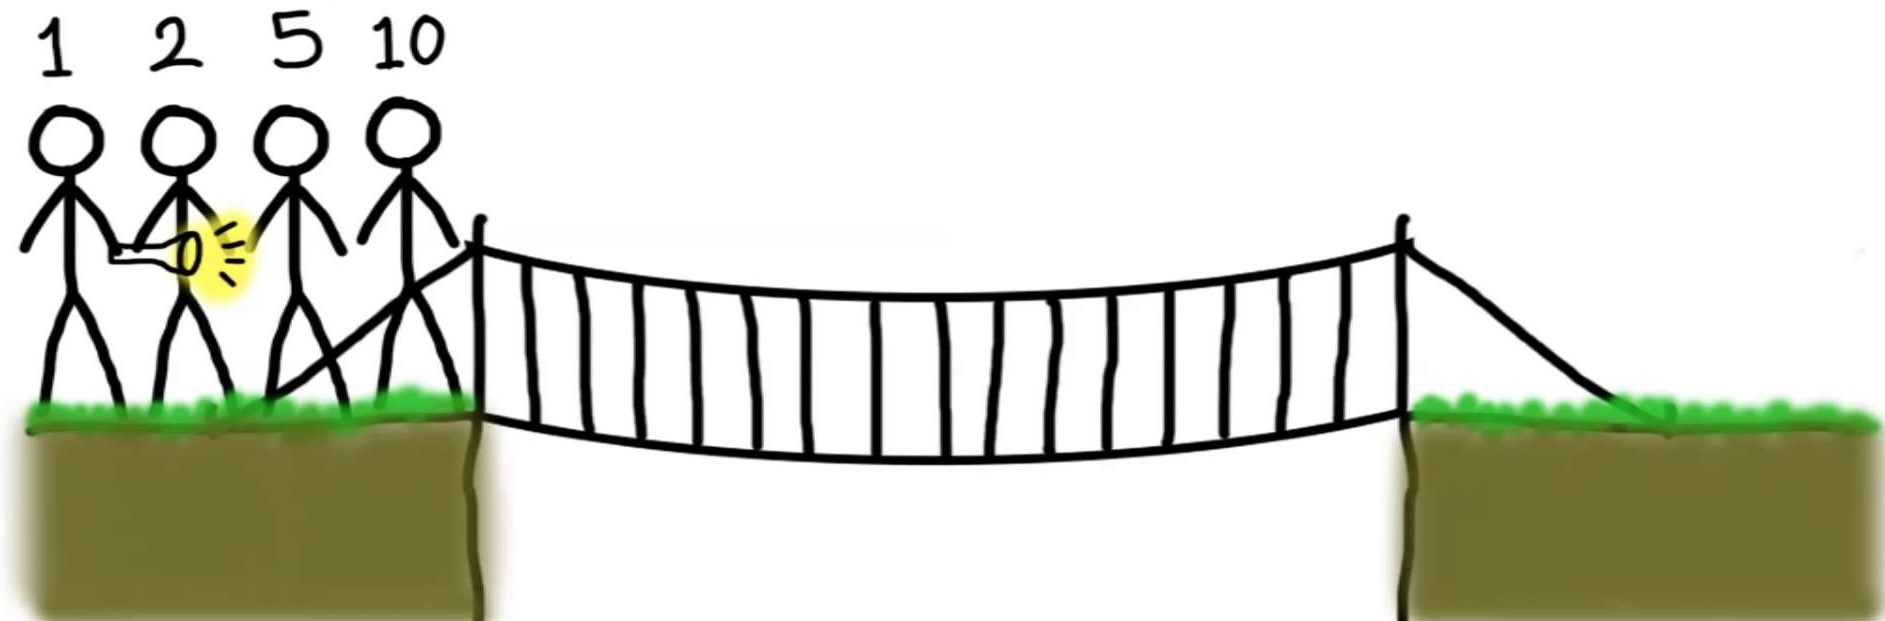
\includegraphics[width=5cm]{bridge.jpg}
\captionof{figure}{Tilts pāri aizai}
\label{fig:bridge}
\end{center}
\end{problem}
%

%2
\begin{problem}
\textit{[9 punkti - "domāt ārpus rāmjiem"]}
Uz papīra uzzīmēti $9$ punkti $3 \times 3$ kvadrātrežģa izkārtojumā. Vai ir iespējams uzzīmēt $4$ taisnus un savienotus nogriežņus, kas noklātu visus punktus, neatraujot zīmuli no papīra?
\begin{center}

\includegraphics[width=1.5cm]{3by3.jpg}
\captionof{figure}{9 punkti}
\label{fig:bridge}
\end{center}
\end{problem}
%

%3
\begin{problem}
\textit{[Vēl punkti- "redukcija","domāt ārpus rāmjiem"]}
Tas pats, kas iepriekšējā uzdevumā, bet:
\begin{enumerate}
\begin{multicols}{2}
\item $5 \times 5$ ar $8$. nogriežņiem 
\item $4 \times 4$ ar $6$. nogriežņiem
\item $3 \times 4$ ar $5$. nogriežņiem
\item $4 \times 5$ ar $7$. nogriežņiem
\end{multicols}
\end{enumerate}
\end{problem}
%

%4
\begin{problem}
\textit{[Sultāna likums - "simetrija"]}
Sultanātā ir vienāds skaits sieviešu un vīriešu, bet, reliģiskas pārliecības vadīts, Sultāns gribētu, lai sieviešu būtu vairāk nekā vīriešu.
Viņam ir padomā sekojošs likums - katrai sievietei jādzemdē bērni līdz viņa piedzemdē pirmo dēlu, bet pēc tam vairāk bērnus dzemdēt nedrīkst.

Vai šāds likums panāktu to, ka sieviešu ir vairāk nekā vīriešu? Un kas notiktu ar vidējo bērnu skaitu katrai mātei Sultanātā?
\end{problem}
%


%5
\begin{problem}
\textit{[Azartspēļu problēma - "simetrija"]}
Elīzei un Rūdolfam matemātikas stundā kļuva garlaicīgi un viņi izdomāja izklaidēties ar sekojošu azartspēli. Katrs no viņiem sākumā izvēlas trīs notikumu - monēta vai ģerbonis - secību un tad viņi met godīgu monētu līdz šajā metienu sērijā sastopas kāda no izvēlētajām virknēm, un, attiecīgi, tās minētājs arī uzvar. Nosakiet, kurās no šīm spēlēm abiem ir vienāda iespēja uzvarēt:
\begin{enumerate}

\item "cipars-cipars-cipars" pret "ģerbonis-ģerbonis-ģerbonis"
\item "cipars-cipars-cipars" pret "cipars-cipars-ģerbonis"
\item "ģerbonis-ģerbonis-cipars" pret "cipars-cipars-ģerbonis"
\item "ģerbonis-ģerbonis-cipars" pret "cipars-cipars-cipars"

\end{enumerate}

\end{problem}
%
\end{document}
